\chapter{Introduction to load balancing and RAID controllers}
\label{chap2:title}
\nomenclature{RAID}{Redundant Array of Independent Disks}
\nomenclature{ATA}{Serial ATA (AT Attachment)}
\nomenclature{IDE}{Integrated Drive Electronics}
\nomenclature{SAS}{Serial attached SCSI}
\nomenclature{SMART}{Self-Monitoring, Analysis and Reporting Technology}
\nomenclature{JBOD}{Just a Bunch of Disks}


\section{Load balancing}

In general load balancing is the methodology which increases the speed by balancing the resources. The main idea is to do as much as possible with least amount of resources. Mostly it depends on the processes, which we can divide by threads and launch them parallel. Sometimes load balancing is divided to the 4 types: static, dynamic, combined and preemptive. In scientific articles combined and preemptive load balancing systems are mentioned very rarely because of their specificity and usefulness only in some certain cases. That is why in this research it will be considered 2 main different types: static and dynamic.
% combined? (http://masters.donntu.edu.ua/2011/fknt/baluta/library/article1.htm)
% preemptive? (http://dictionary.reference.com/browse/load+balancing)


Static load balancing system makes the analysis before the application starts. That is why for creating good load balancing system via static methods the programmer should know several pieces of information. Firstly, the amount of distributed work should be well known before the program is written. And secondly, the duration of the tasks to be divided should be approximately the same. There are several methods to hand out the tasks such as Round Robin algorithm, Random algorithm, Recursive Bisection algorithm and some others \cite{oper_sys_conc}, \cite{perf_dlba}. Frequently the initial parameters are taken from the previous launch results and genetic algorithms are used. An example of load balancing system can be taken from image processing. Let consider 16$\times$16 segmented image and 8 processors. With that image each processor would work on 4 segments. The most important piece of all this division of work is that each processor determines this information and also which segments it will work on.


Dynamic load balancing systems have more possibilities because the balancing process can be done during the application running \cite{guide_dyn_bal}. This fact gives the advantage of resource movement from busy part to less busy, that all of the parts of the application will be in average busy condition. The disadvantage of that method is that the system should also collect the information about the condition of application, which follows the increasing of the resources. There are 3 general criteria, which programmer should follow during making the dynamic load balancing system:
\begin{enumerate}%[topsep=0pt, itemsep=-0.5ex]
	\setlength{\itemsep}{-2mm}
%	\setlength{\topsep}{-10mm}
	\item Which process is busy or free 
	\item Priority of the task to be done 
	\item Length and/or duration of the task
\end{enumerate}
The program, which realized the dynamic load balancing system, should check the loading of computation units, connection possibility and frequency of sending commands. Dynamic load balancing methodology has a lot of methods, such as Bidding algorithm, Drafting algorithm, Recursive Coordinate Bisection (RCB) and some others. In scientific papers they can be called as strategies and policies, but in the following content it will be called methods.



\section{RAID}
RAID - Redundant Array of Independent Disks - is a storage technology that combines multiple disk drive components into a logical unit. That means that this technology gives a possibility to keep the information in a specific way. RAID controllers are the devices, which realize this technology. In simple words without a RAID controller computer can see physical disks as a logical disks without any difference. But with RAID controller the computer will see only the logical disks, which will be definitely different in comparison in physical disks. All issues about creation of these logical disks are taken by RAID controller.

There are several types of RAID: RAID 0, RAID 1, RAID 5, RAID 6 and some others \cite{which_raid}. These types of RAID, which were mentioned, are basic types of RAID, thus there are many other types, which also combine them together. For example, RAID 10 is actually combining of RAID 0 and RAID 1. Each type or architecture provides a different balance between the key goals: reliability and availability, performance, and capacity. That means that every RAID keeps the information in a different way. 

One of the huge advantages of using RAID is that if one of the disks breaks down others can recover the information on that disk. Not all RAID architectures supports this functionality, but most of them do. Some types of RAID provide fault tolerance of even two drive failures (RAID 6).

Let consider some types of RAID more detailed. RAID 1 called also as "mirroring" is one of the main fundamental types of RAID, which refers to maintaining duplicate sets of all data on separate disk drives. There must be two disks in the configuration and there is a cost disadvantage as the usable
capacity is half the number of available disks. RAID 1 provides cost-effective, high fault tolerance for configurations with two disk drives. The prototype of RAID 1 is presented on the figure \ref{fig:raid1}.
\begin{figure}[h]
\begin{center}
  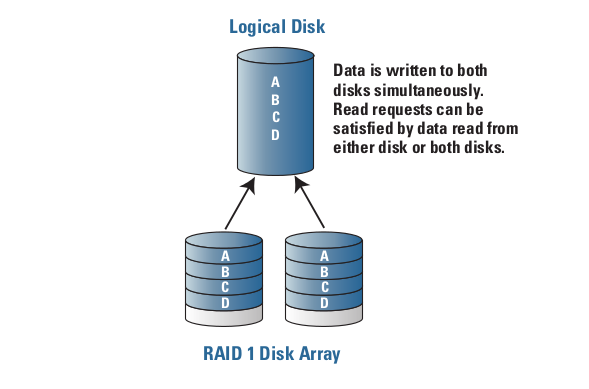
\includegraphics[width=0.95\textwidth]{raid1}
\end{center}
  \caption{Prototype of RAID 1}
  \label{fig:raid1}
\end{figure}

Another type RAID 5 uses data striping in a technique designed to provide fault-tolerant data storage, but doesn't require duplication of data like RAID 1 \cite{raid_overview}. Data is striped across all of the drives in the array, but for each stripe through the array (one stripe unit from each disk) one stripe unit is reserved to hold parity data calculated from the other stripe units in the same stripe. Read performance is therefore very good, but there is a penalty for writes, since the parity data has to be recalculated and written along with the new data. RAID 5 requires a minimum of three disks and a maximum of 16 disks to be implemented. RAID 5 usable capacity is between 67\% - 97\% depending on the number of data drives in the RAID set.
\begin{figure}[h]
\begin{center}
  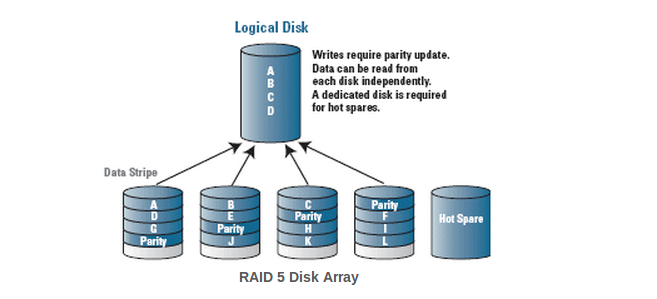
\includegraphics[width=0.95\textwidth]{raid5}
\end{center}
  \caption{Prototype of RAID 5}
  \label{fig:raid5}
\end{figure}



Moreover, nowadays there are RAID controllers, which already have load balancing system inside and the user can set the mode, which is more comfortable in the some situations. In our case the commands should be sent straight to the disk that is why the load balancing system from controller is not helping at all, because of its own methodology.  


On the picture \ref{fig:3ware_RAID} one of the SATA RAID controllers is presented. 
\begin{figure}[h]
\begin{center}
  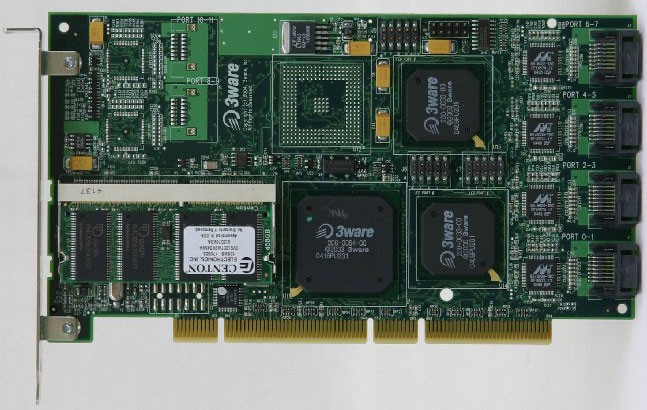
\includegraphics[width=0.95\textwidth]{3ware_RAID}
\end{center}
  \caption{3ware SATA RAID controller 9500S-8}
  \label{fig:3ware_RAID}
\end{figure}
From the name of the device it is clear that this controller can be connected to 8 SATA disks. It supports following types of RAID: 0, 1, 5, 10, 50 and JBOD (Just a Bunch of Disks).



\section{SCSI RAID controllers}
SCSI - Small Computer System Interface - is a set of standards for physically connecting and transferring data between computers and peripheral devices \cite{book_of_scsi}. The SCSI standards define commands, protocols, and electrical and optical interfaces. There are also other interfaces such as SATA (Serial ATA (AT Attachment)), IDE (Integrated Drive Electronics), SAS(Serial attached SCSI). In general, the interfaces are divided by two categories: ATA and SCSI. In the following content it means the according protocol. IDE and SATA interfaces are related to ATA and SAS is related to SCSI. Several types of disks are presented on the figure \ref{fig:disks}. In this paper the topic mostly is about SCSI interface, but sometimes it will be compared with ATA. If SAS and SCSI are compared, it can be considered similar interfaces. However, SAS is a new version of SCSI and it gives a single channel for each disk. In comparison with SCSI it was only one channel for all disks.
\begin{figure}[h]
  \advance\leftskip-0.1\textwidth
  \subfloat[SCSI disk]{
    \label{fig:scsi}
    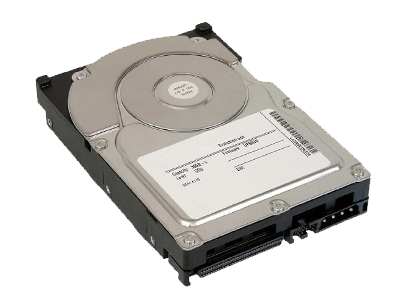
\includegraphics[width=0.6\textwidth]{scsi}
  }
  \subfloat[SATA and IDE disks]{
    \label{fig:sata_ide_disks}
    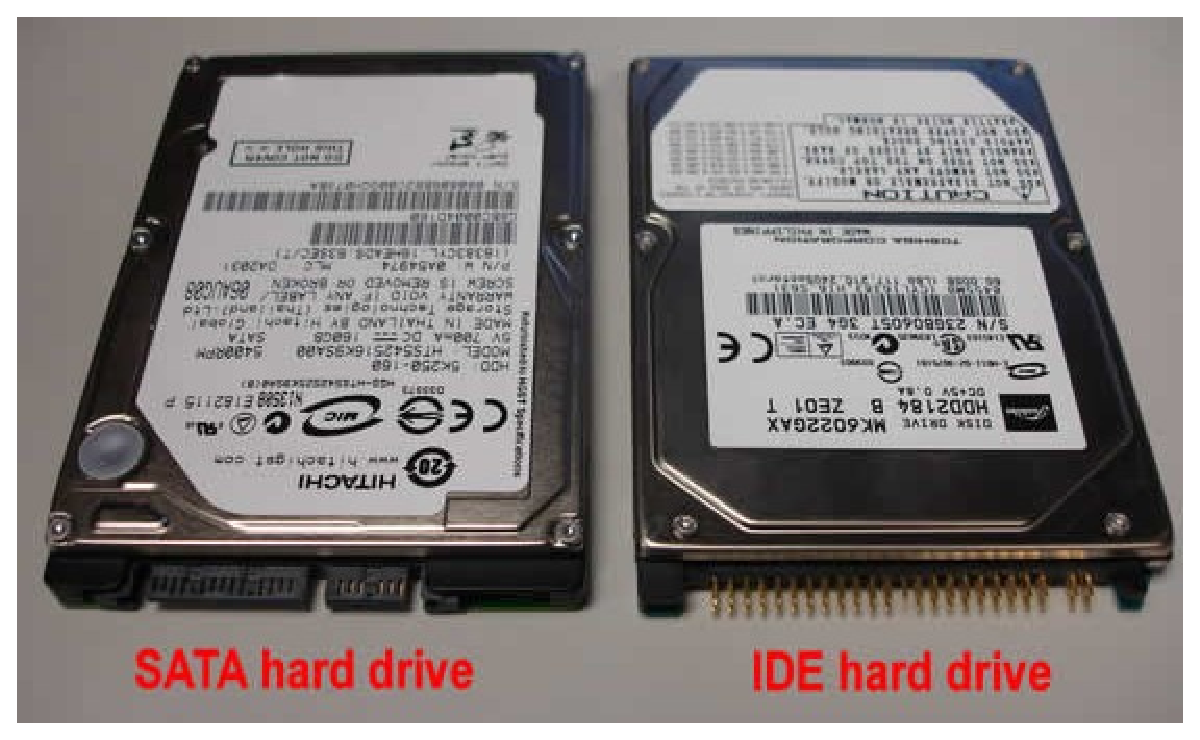
\includegraphics[width=0.6\textwidth]{sata_ide_disks}
  }
  \caption{Three different types of disks}
  \label{fig:disks}
\end{figure}




\section{SCSI WRITE and WRITE SAME commands}
\label{subsec:write_comm}
This research is made for the Blancco Oy Ltd, which produce the erasure software. The main part of the erasure is performed by SCSI WRITE and WRITE SAME commands \cite{scsi3_bc}. In general, all commands are divided to three groups: Non-Data commands, Data-In and Data-Out. For the last two groups it means that the command is sent including the buffer. Data-Out means that the data is sent to the disk. For the Data-In group it is in opposite way and data is come from the disk. The example of Data-In command is any SCSI READ command. Write commands are related to the Data-Out group because these commands must have Data-Out buffer, containing the data, which will be written to the disk. Nowadays, for SCSI there are 4 different versions of write command and 3 for the write same command.  

Lets consider SCSI write commands first. Mostly the commands are different because of the length. Each command has not only operation code, which is the main criteria for the command, but also some other variables such as Logical Block Address (LBA), transfer length, control and some others. These variables do not include Data-Out buffer and the Figure \ref{fig:write_10} shows the example how the commands are defined in specification \cite{scsi3_bc}.
\begin{figure}[h]
\begin{center}
  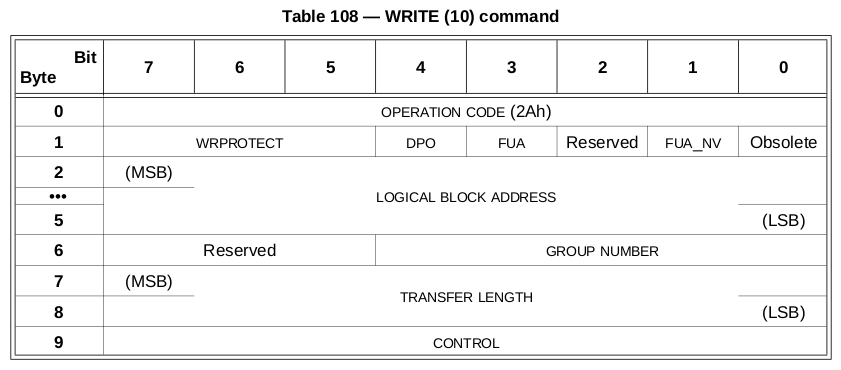
\includegraphics[width=0.95\textwidth]{write_10}
\end{center}
  \caption{Definition of WRITE 10 command}
  \label{fig:write_10}
\end{figure}


The following commands exist for writing the data to the disk:
\begin{itemize}%[topsep=0pt, itemsep=-0.5ex]
	\setlength{\itemsep}{-2mm}
%	\setlength{\topsep}{-10mm}
	\item WRITE (10)
	\item WRITE (12)
	\item WRITE (16)
	\item WRITE (32)
\end{itemize}
The numbers in brackets shows the length of the command in bytes. It is obvious that the WRITE (10) command is the base for others. It seems that by now the best choice is WRITE (16) because in \cite{scsi3_bc} there are some notes, that <<Migration from the WRITE (10) command to the WRITE (16) command is recommended for all implementations>>. WRITE (32) should be used only in some special cases \cite{scsi3_bc}.

SCSI write same commands have the same purposes as SCSI write commands. The difference and biggest advantage is that SCSI write same command can be sent once and the Data-Out buffer can be written to the disk several times. That gives faster speed because the bus is not busy any more - only one command was sending, but the buffer is still writing. 
There are 3 different types of write same commands, as it was noticed before:
\begin{itemize}%[topsep=0pt, itemsep=-0.5ex]
	\setlength{\itemsep}{-2mm}
%	\setlength{\topsep}{-10mm}
	\item WRITE SAME(10)
	\item WRITE SAME(16)
	\item WRITE SAME(32)
\end{itemize}
The number in brackets also shows the length of the command in bytes. Number of logical blocks is one of the most important variable in these commands because this number of blocks will be written to the disk with the same buffer. It is obvious that as bigger is the length of the SCSI write same command as more number of blocks we can write to the disk. ATA has the similar command, but it should be send differently and the device should support SMART (Self-Monitoring, Analysis and Reporting Technology) \cite{ata_spec}. It is a monitoring system for computer hard disk drives to detect and report on various indicators of reliability.





